\documentclass[12pt,svgnames]{report}
\usepackage{tikz}
\usepackage{verbatim}
\usepackage[margin=1.1in]{geometry}
\usepackage{booktabs}
\usepackage{graphicx}
\usepackage{hyperref}
\usepackage{kpfonts}
 \usepackage{url}
\usepackage[explicit]{titlesec}
\usepackage{xcolor}
\usepackage{sectsty}
\definecolor{mycolor}{HTML}{0059b3}
\definecolor{mycolor2}{HTML}{0066cc}
\sectionfont{\color{mycolor}}
\subsectionfont{\color{mycolor2}}
\subsubsectionfont{\color{mycolor2}}
\newcommand*\chapterlabel{}
\titleformat{\chapter}
{\gdef\chapterlabel{}
	\normalfont\sffamily\Huge\bfseries\scshape}
{\gdef\chapterlabel{\thechapter\ }}{0pt}
{\begin{tikzpicture}[remember picture,overlay]
	\node[yshift=-1cm] at (current page.north west) %poso paxi tha einai to mple rectangle
	{\begin{tikzpicture}[remember picture, overlay]
		\draw[fill=MidnightBlue] (0,-1) rectangle
		(\paperwidth,2cm);
		\node[anchor=west,xshift=.1\paperwidth,rectangle,
		rounded corners=15pt,inner sep=9pt,
		fill=MidnightBlue]
		{\color{white}\chapterlabel#1};
		\end{tikzpicture}
	};
\end{tikzpicture}
}
\titlespacing*{\chapter}{0pt}{50pt}{-60pt}

\title{\color{mycolor}Report on Twitter topic detection and analysis}
\author{
Alex Tsilingiris \\
Christina Pardalidou \\
Sotiris Karapostolakis \\
}

\begin{document}
\maketitle
\begingroup
\color{mycolor}
\tableofcontents
\endgroup
\chapter{Introduction}
To keimeno sth sinexeia einai mia texniki anafora tou tade project to opoio ekane auta k auta me vash auta. stoxos itan auto k auto kai gia tin diekpaireosh tou egine auto k auto.

\chapter{Method implementation details}
\section*{Event detection}
\subsection*{Our approach}
A combination of approaches was used for event detection: Since the dataset was static and filtered based on a query (in our case the word "trump"), terms were considered as living organisms in the given timespan, allowing us to sample a set of tweets as when each term was "most alive", while combining user reputation metrics to select a tweet from a reputable source.
\subsubsection*{Hashtags as terms}
We solely operated on hashtags on this step since they represent an idea or a topic, which in other cases would be difficult, or not as accurate, to define using Natural Language Processing and Machine Learning.
\subsubsection*{The living organism implementation}
We considered a term as most-alive at the point in which it was mostly detected in our dataset. The time window was set to 2 hours. Therefore, we had to query for the mostly found terms (using the Term Frequency statistic) and sort the results in descending order. We then generated the final that contained the original tweets with the most active terms in the dataset that were posted in the given timespan.
\subsubsection*{Selecting a tweet from the pool}
We now have a pool of tweets that might contain information about an event. The approach we followed was to assume that a user with a high amount of followers represents an influential event source  into a social community\cite{cataldi2013personalized}. We sorted (descending) the tweet pool by the number of followers the original poster has and ended up with 1 tweet that was our result for each term.
\section*{Sentiment Analysis}

\subsection*{Methodology}
For the prediction of the sentiments of the tweets gathered, we used a supervised method. In particular, we used a machine-learning technique. The tool we used for the predictions was implemented for the needs of a course in the previous semester. Since we had put a lot of effort in its implementation and it is a creation of our personal hard work we decided to use it for this assignment too.

\subsubsection*{Selecting tweets from the dataset}
All the tweets related to the top emerging event were isolated and written to different text files. These are all the tweets that include hashtags related to the event (e.g \#parisagreement). All the retweets  were removed. 

\subsubsection*{Sentiment Prediction}
The Opinion-Mining tool\cite{opinion} we used implements a SVM classifier that classifies the tweets in two categories: positive and negative. SVM performs very well and is considered as one of the top performing classifiers in the literature. This tool is further presented in \autoref{chap:framework}.

\chapter{Framework description}
\label{chap:framework}
The software created was split into modules to allow for independent, on-demand functionality. A user can easily assemble a system from these independent modules based on their needs. The complete repository can be found in the project's Github page \cite{projectgithub}.
\subsubsection*{Getting the tweets}
To begin with, Python and Tweepy \cite{tweepy} were used to access the Twitter API as efficiently as possible. The incoming stream was filter using the keyword "trump" and was directly saved into a MongoDb instance.

\subsubsection*{Preprocessing the dataset}
A custom preprocessing module was created to combine all the required steps needed when analyzing tweets. The nltk \cite{nltk} library along with some custom regular expressions were used in order to complete the following actions: group hashtag symbols with the hashtag word, group mention symbols with the mention target, keep URLs functional and finally remove stop-words, punctuation and twitter specifics such as "via" and "rt". Finally, a script was created to convert datetime strings into MongoDb specific datetime strings so that range queries were possible.

\subsubsection*{Plotting}
The pandas \cite{pandas} library was used to resample the time and allow tweet bucketing based on a given time window. The window size used for term (hashtag) visualization was 120minutes. The results were exported directly into .json format and are presented in our website \cite{projectwebsite} using the d3js \cite{d3js} library.

\subsubsection*{Getting the tweets for sentiment analysis}
After detecting the top event that occurred during the time the tweets were crawled, the dataset was filtered in order to get only the tweets, without the retweets, containing hashtags related to the emerging event (e.g \#parisagreement, \#climatechange). These specific tweets were written to text files so they can be imported to the Opinion-Mining tool\cite{opinion} for sentiment prediction.

\subsubsection{Opinion-Mining tool}
The tool uses a custom lexicon implementation that is shown in figure \ref{fig:opinion}. The training set used includes a total of 25k labeled reviews taken from the published dataset of IMDb \cite{imdb}. Half of them are positive and the other half are negative.
\begin{figure}[h]
	\centering
	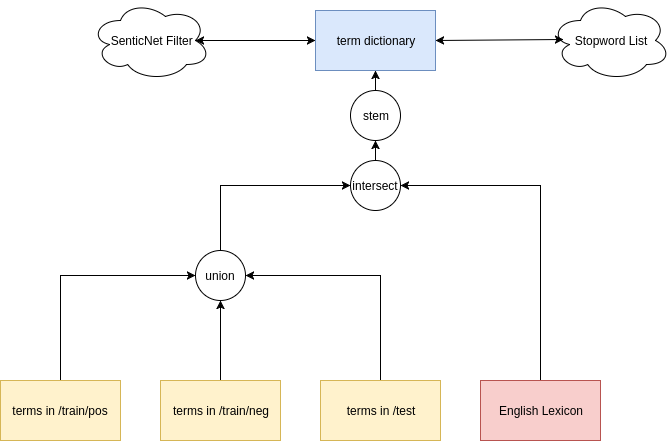
\includegraphics{opinion}
	\caption{Depiction of the diagram of the lexicon.}
	\label{fig:opinion}
\end{figure}

\subsubsection{Preprocessing process}
\begin{itemize}
	\item Punctuation removal, tokenization.
	\item Stemming (non-English terms are deleted).
	\item Terms frequencies.
	\item TF/IDF Vectors.
\end{itemize}

\subsubsection{Prediction}
The model uses a SVM classifier with SGD tuning for prediction. The vectors are defined with TF: log normalized and IDF: smooth normalized. The output is a text file that has in each row the name of the input text file and the output of the prediction for this file i.e 1.0 for positive and 0.0 for negative tweets.

\chapter{Results}
\section*{Event detection}
Some top ranked terms (hashtags), their occurrences and the tweet that qualified as an event by our system will be presented in table \ref{tab:tftags}

\begin{table}[h!]
	\centering

	\begin{tabular}{ccc}
		\toprule
		Term & Frequency\\
		\midrule
		\#parisagreement & 10442\\
		\#covfefe & 7085\\
		\#trumprussia & 4229\\
		\#marchfortruth & 973\\
		\bottomrule
	\end{tabular}
	\caption{Terms and occurrences}
\label{tab:tftags}
\end{table}


A graph showing the top ranked term's occurrence over time can be seen in the following figure:\\
\\
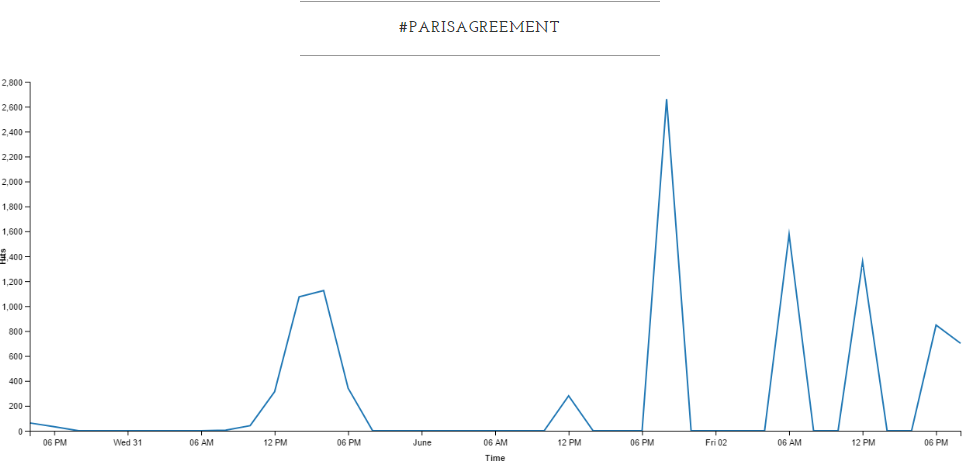
\includegraphics[scale=0.63]{hashparisplot.png}
\\

\newpage
The tweet that our system determined as an event can be seen in the following figure:
\begin{figure}[h]
\centering
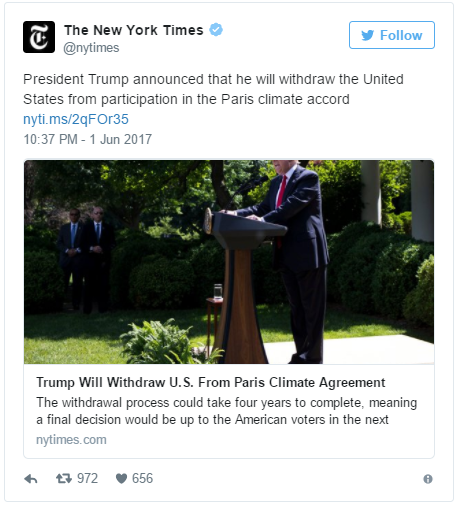
\includegraphics[scale=1]{hashparistweet.png}
\end{figure}
\\
Additional results can be found in the project's website \cite{projectwebsite}.

\section*{Sentiment Analysis}
The predictions of the sentiments of the tweets are presented using a pie chart in \ref{fig:pie_chart}. The number of tweets that corresponds to each sentiment is presented in Table \ref{tab:sentis}.

\begin{table}[h!]
	\centering	
	\begin{tabular}{ccc}
		\toprule
		Opinion & Number of tweets\\
		\midrule
		Negative & 1501\\
		Positive & 1183\\		
		\bottomrule
		Total & 2684
	\end{tabular}
	\caption{Predictions of the tweets}
	\label{tab:sentis}
\end{table}

\begin{figure}[h]
	\centering
	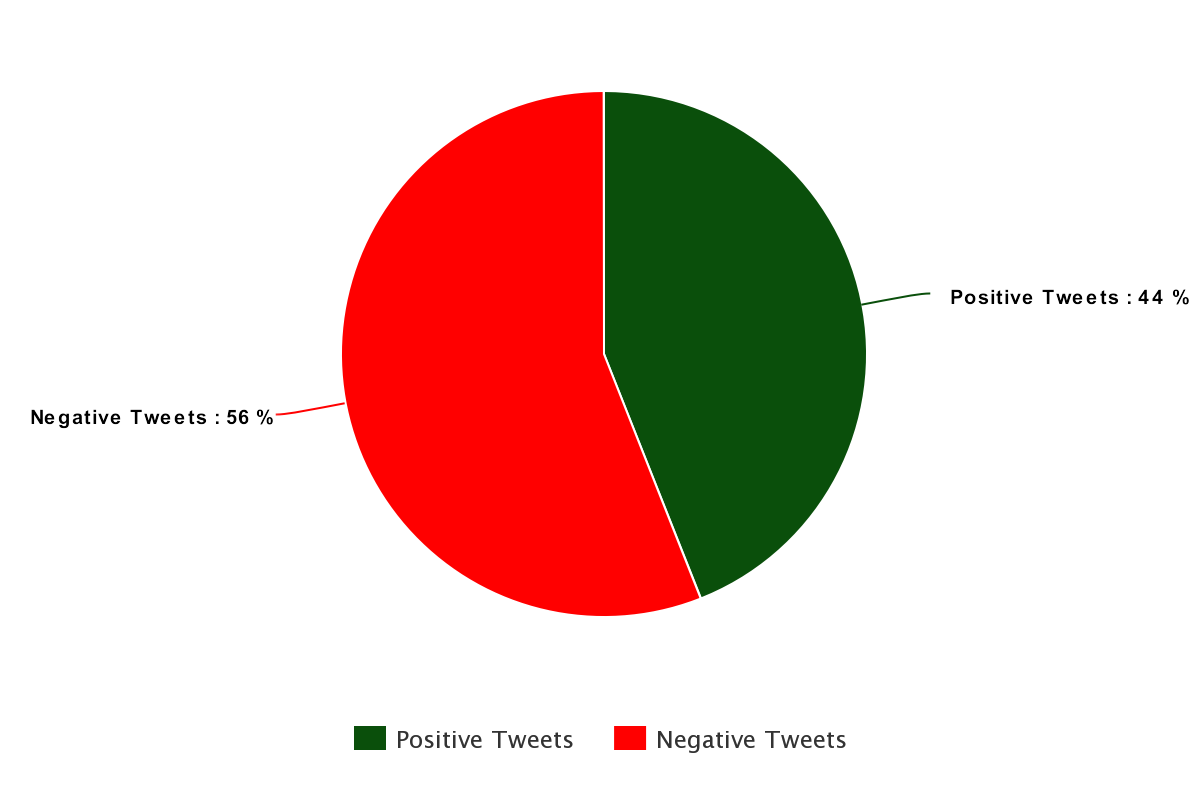
\includegraphics[scale=0.6]{pie_chart}
	\caption{Percentages of negative and positive tweets.}
	\label{fig:pie_chart}
\end{figure}


\addcontentsline{toc}{chapter}{5\:\:\: Bibliography}
\bibliographystyle{abbrv}
\bibliography{sigproc}
\end{document}